\section{W1: Use Case Diagrams}
\textbf{Actors:} A person or a system that interacts with the system.\\
\begin{itemize}
    \item \textbf{Primary actor:} initiates the use case. Has goals that influences the purpose of the system under discussion (SuD).
    \item \textbf{Supporting actor:} provides a service to the SuD, like a dependency.
    \item \textbf{Offstage actor:} interacts with the SuD, but is not part of the SuD. Almost like a spectator.
\end{itemize}
\textbf{Use case:} a sequence of actions that provide a measurable value to an actor.\\
\textbf{Use case diagram:} a diagram that shows the actors and use cases of a system.\\
\textbf{How to find useful use cases?}
\begin{itemize}
    \item \textbf{Boss test:} if I told my boss about this use case, would he/she care?
    \item \textbf{Elementary business process (EBP):} a task that is performed by one person, in one place, in response to a business event, and adds measurable business value.
    \item \textbf{Size test:} is a task very seldom a single action/step?
\end{itemize}
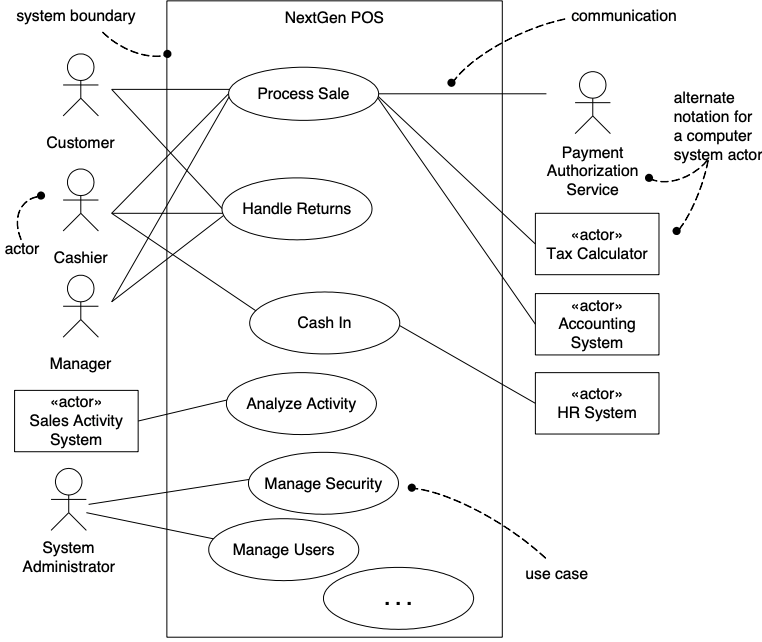
\includegraphics[width=\linewidth]{figs/uml-use-case-diagram.png}